\section{Metodologija}

\subsection{Opis referentne aplikacije}

Za potrebe testiranja performansi različitih programskih okvira kroz različite strategije iscrtavanja bilo je potrebno napraviti demo aplikaciju koja bi bila reprezentativna, ali ne presložena, te bi uključivala stranice sa statičnim i dinamičnim sadržajem.

\bigskip

Predstavnik statične stranice je stranica „O nama“. Ovakve stranice najčešće koriste statičan sadržaj koji se vrlo rijetko mijenja, te često čine dio web aplikacija raznih tvrtki. Dinamični dio predstavljaju stranice bloga, također popularnog sadržaja na webu.

\bigskip

Kako bi se održala konzistentnost implementacije u svim programskim okvirima navedene stranice imaju istu strukturu (HTML) i za stiliziranje koriste Tailwind CSS okvir koji je vrlo popularan i raširen zbog svoje jednostavnosti korištenja i integracije sa modernim programskim okvirima.

\bigskip

Za font je korišten Google font obitelji Archivo. Sve slike osim open graph sike poslužuju se kroz servis Lorem Picsum prema id-ju ili seedu kako bi se izbjeglo učitavanje nasumičnih slika pri svakoj posjeti stranice. Za dohvaćanje sadržaja bloga korišten je popularni servis za posluživanje testnih podataka JSONPlaceholder.

\bigskip

\begin{figure}[H]
    \centering
    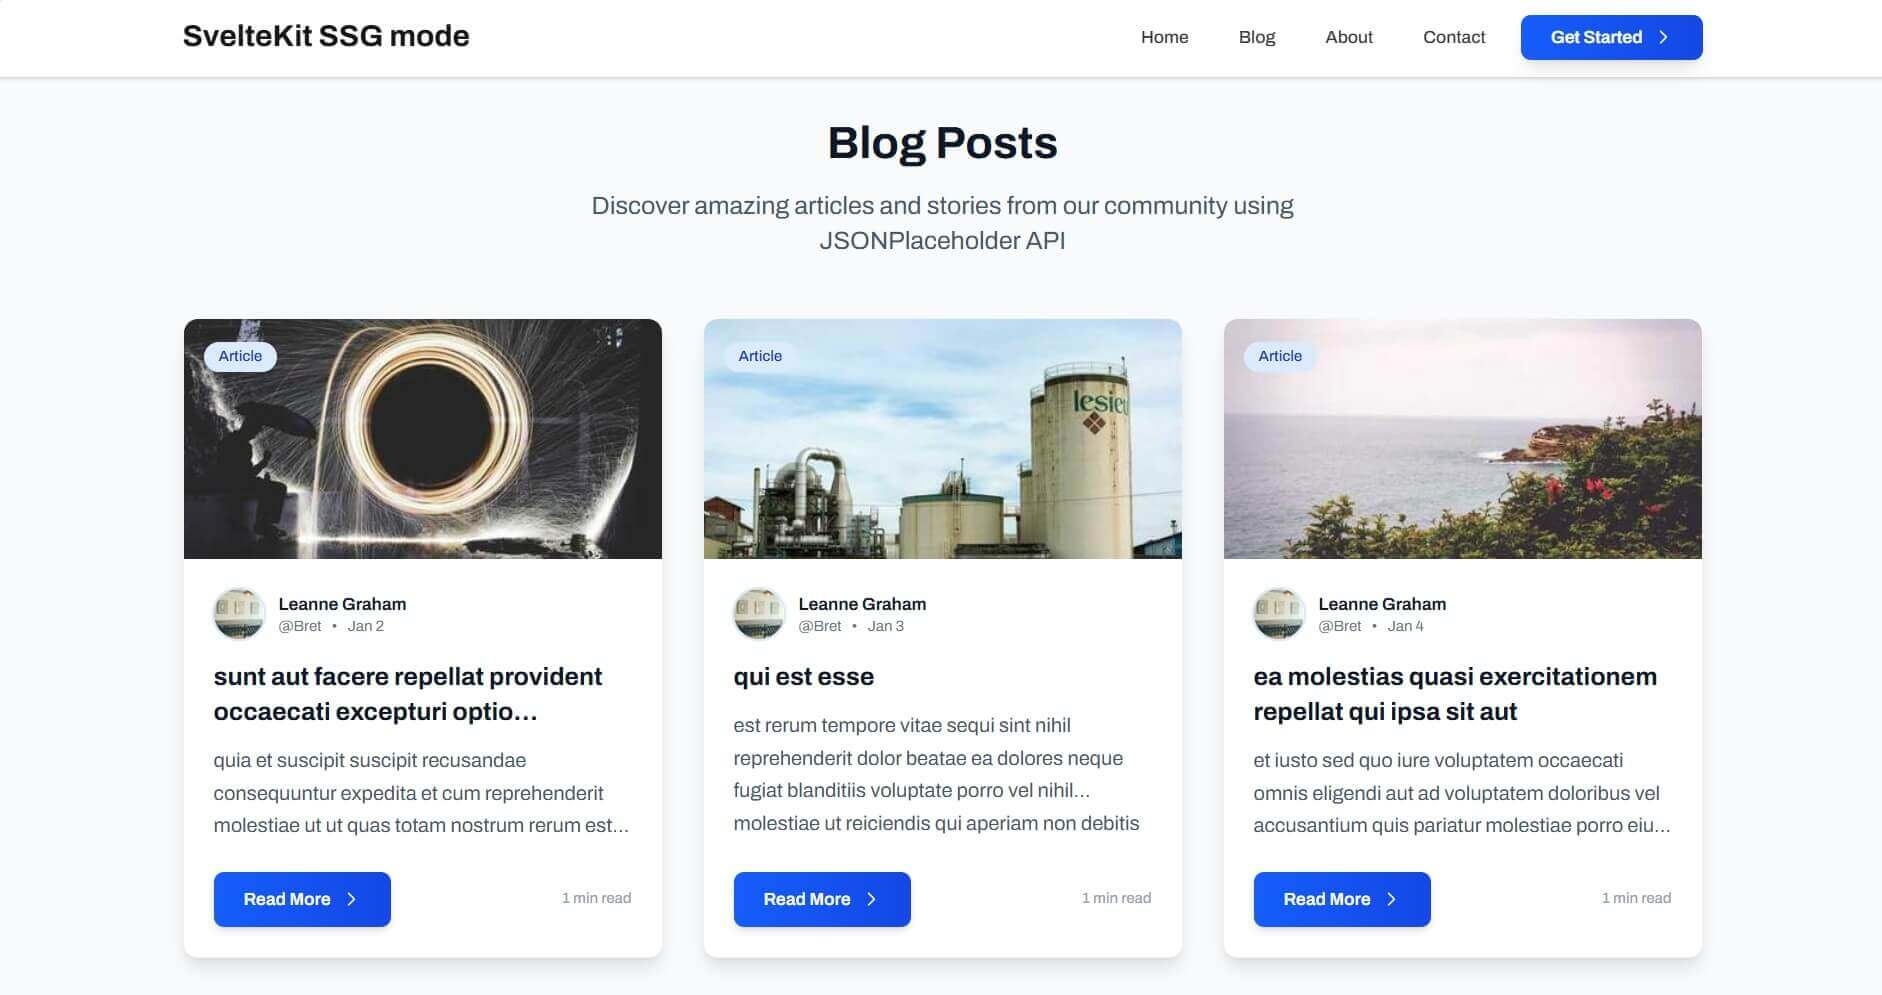
\includegraphics[width=\textwidth]{slike/metodologija/prikaz-blog-stranice.jpg}
    \caption{Prikaz blog podstranice}
    \label{fig:prikaz-blog-stranice}
\end{figure}

\subsection{Implementacija u programskim okvirima}
Work in progress
% TODO ovo poglavlje napisati

\subsection{Mjerene metrike Performansi}

Za mjerenje performansi aplikacije odabrane su standardne metrike poznate pod nazivom Web vitals nastale na Googleovu inicijativu kako bi se standardiziralo mjerenje performansi i dobio bolji uvid u korisničko iskustvo. Osim glavnih metrika u istraživanje su uključene i dodatne metrike poput vremena izgradnje, vremena skriptiranja i veličine JavaScript paketa koji se dostavlja klijentu. Slijedi kratak pregled svih korištenih metrika.

\subsection{Iscrtavanje najvećeg sadržaja (LCP)}

LCP, odnosno „Largest Contentful Paint“, mjeri koliko je vremena potrebno da se na stranici prikaže njen najveći vidljivi element. Proteklo vrijeme do 2,5 sekunde smatra se dobrim pokazateljem performansi. U obzir se uzima samo onaj dio elementa koji korisnik može vidjeti – dijelovi koji su odrezani ili nisu vidljivi se zanemaruju. Tijekom učitavanja stranice, koje se često odvija u nekoliko koraka, taj najveći element može se promijeniti. Prvo se zabilježi vrijeme učitavanja tada najvećeg elementa, a ako se kasnije pojavi još veći, mjeri se vrijeme učitavanja novog elementa. Kada korisnik počne koristiti stranicu, preglednik prestaje pratiti nove elemente jer interakcije mogu promijeniti ono što je vidljivo. LCP se zato koristi kao pokazatelj trenutka kada je glavni sadržaj stranice postao dostupan korisniku \cite{nordstrom2023comparison}.

\subsection{Ukupno vrijeme blokiranja (TBT)}

TBT (engl. Total Blocking Time) predstavlja ukupan vremenski period koji protekne od otvaranja stranice do trenutka kada korisnik može normalno stupiti u interakciju s njom. Pod interakcijom se podrazumijevaju radnje poput klika mišem, dodira zaslona ili unosa putem tipkovnice. Vrijeme se računa tako da se zbroje svi dijelovi dugih zadataka (onih koji traju više od 50 milisekundi), a koji sprječavaju preglednik da odmah odgovori na korisničke radnje. Ovi se zadaci bilježe u razdoblju između početnog prikaza sadržaja (FCP) i trenutka kada stranica postane potpuno funkcionalna. Sve što prelazi granicu od 50 ms kod pojedinog zadatka ulazi u ukupnu vrijednost TBT-a \cite{nordstrom2023comparison}.

\subsection{Kumulativna promjena rasporeda (CLS)}

Pomicanje sadržaja na web stranici tijekom njenog učitavanja naziva se  pomak izgleda (engl. layout shift). Do toga najčešće dolazi zbog asinkronog učitavanja sadržaja ili dodavanja novih DOM elemenata preko postojećih komponenti. CLS prati najveći niz takvih pomaka koji se dogode unutar jednog vremenskog okvira od maksimalno 5 sekundi, pri čemu između pojedinih pomaka ne smije proći više od jedne sekunde. Ova metrike je važna jer pokazuje stabilnost stranice, a poželjno je da rezultat bude što niži – vrijednost 0.1 smatra se dobrim rezultatom \cite{nordstrom2023comparison}.

\subsection{Vrijeme do interaktivnosti (TTI)}

Ova metrika označava koliko je vremena potrebno da web stranica postane potpuno interaktivna. To znači da se prvo prikaže koristan sadržaj (što mjeri FCP), zatim da stranica reagira na korisničke radnje u roku kraćem od 50 milisekundi te da je većina upravljača događaja (engl. event handler) učitana i spremna. Vrijeme kraće od 3,8 sekundi smatra se dobrim rezultatom. Spor TTI često je uzrokovan loše optimiziranim JavaScript kodom. \cite{nordstrom2023comparison}

\subsection{Vrijeme do prvog bajta (TTFB)}

Vrijeme do prvog bajta označava koliko vremena prođe od trenutka kada preglednik pošalje zahtjev prema serveru do trenutka kada primi prvi bajt povratnog odgovora. Ova metrika prikazuje koliko brzo se uspostavlja veza i koliko brzo server reagira, uključujući sve faze poput preusmjeravanja, DNS rezolucije, TLS dogovora i slanja zahtjeva. Niža vrijednost TTFB-a znači da se stranica učitava brže, što pozitivno utječe i na ostale važne metrike poput FCP-a. Idealno bi bilo da TTFB ostane ispod 0,8 sekundi radi optimalnog korisničkog iskustva \cite{pollardttfb}.

\subsection{Dodatne metrike}

\begin{itemize}
    \item Veličina paketa (engl. bundle size) predstavlja ukupnu veličinu svih JavaScript datoteka koje se preuzimaju prilikom početnog učitavanja stranice – uključujući sve JS dijelove potrebne za prikaz početne stranice.
    \item Vrijeme izgradnje (engl. build time) odnosi se na trajanje procesa generiranja statičkih stranica prilikom pretvaranja izvornog koda u izvršni kod. Vrijeme izgradnje može se očitati iz terminala prilikom lokalne izgradnje ili pak iz Vercelovih zapisa izgradnje (eng. build logs).
    \item Ukupno trajanje izvršavanja skripti (engl. total scripting time) predstavlja zbroj vremena izvršavanja svih JavaScript skripti na stranici. Ova metrika pomaže pri identifikaciji potencijalnih uskih grla u performansama aplikacije.
\end{itemize}


\subsection{Lighthouse}

Glavni i de facto standard za testiranje performansi web aplikacija je Googleov alat otvorenog koda imena Lighthouse. Ovaj alat integriran je u Chrome preglednik, ali i dostupan kao zasebna CLI aplikacija. Pruža sve što je potrebno za provođenje testova performansi i SEO-a i generiranje izvještaja u različitim formatima, što ga čini vrlo funkcionalnim i korisnim u unapređivanju tehničke strane web aplikacija i korisničkog iskustva \cite{googlelighthouse}.

\subsection{Chrome DevTools}

Chrome DevTools je set alata unutar Chrome preglednika koji između ostalog omogućuju analizu performansi web stranice. U kontekstu ovog rada najvažniji su paneli Performance i Network koji prikazuju brzinu učitavanja stranice i resursa. Ključna funkcionalnost je Performance Insights, koja snima korisničku sesiju i bilježi metrike poput FCP i LCP. Ovaj alat korišten je u analizi veličine JavaScript paketa koje klijent preuzima i izvršava \cite{nordstrom2023comparison}.

\subsection{Lighthouse reporter}

Za potrebe ovog rada bilo je potrebno izvesti 360 Lighthouse testova\footnote{3 aplikacije * 4 strategije iscrtavanja * 10 testova po kombinaciji * 3 podstranice (about, blog, blog detalji)} te prikupljene podatke obraditi, grupirati i sažeti (izraditi master tablice sa prosječnim vrijednostima). Zbog opsežnosti testiranja jedini praktični način bilo je napraviti Node.js skriptu koja će na temelju definiranih parametara koristeći Lighthouse CLI alat izvršiti sve testove i generirati datoteke s rezultatima u CSV formatu za daljnju analizu podataka.
Aplikacija za testiranje sastoji se od 3 ključna dijela:
\begin{enumerate}
    \item konfiguracijske JSON datoteke u kojoj su definirani svi parametri testiranja
    \item datoteke LightHouseTestRunner.js koja izvozi istoimenu klasu sa svim metodama važnim za različite načine testiranja
    \item datoteke cli.js koja upravlja testovima i pokreće ih kroz terminal sa odgovarajućim argumentima
\end{enumerate}

Aplikacija za testiranje stavlja korisniku na raspolaganje raznovrstan set testova (prema programskom okviru, prema strategiji iscrtavanja itd.), no za potrebe ovoga rada korištena je naredba koja pokreće testiranje svih aplikacija po određenoj podstranici.

\bigskip

Primjer naredbe u bash terminalu:
\texttt{node cli.js all slow4g blog}

Ova naredba pokreće cli.js skriptu koja testira blog podstranicu u svim aplikacijama u konfiguraciji slow4g.

\bigskip
Skripta će ovom naredbom kreirati sljedeće datoteke za podstranicu blog:
\begin{itemize}
    \item 12 datoteka sa podacima svih 10 mjerenja po programskom okviru i strategiji iscrtavanja
    \item 4 datoteke prosječnih vrijednosti za svaku strategiju iscrtavanja
    \item 1 datoteku sa ukupnim rezultatima za odabranu podstranicu (konačne prosječne vrijednosti svih 12 kombinacija)
\end{itemize}
Ova naredba ponovljena je za svaku podstranicu čime je generirana 51 datoteka\footnote{3 podstranice * 3 programska okvira * 4 strategije iscrtavanja + 12 sažetaka + 3 glavna sažetka}.
Za daljnju analizu korištene su 3 datoteke glavnih sažetaka za svaku stranicu. Svaka od tih datoteka sadrži prosječne vrijednosti testova za svaku od 12 kombinacija strategija i programskih okvira.

\bigskip

Zbog velikog broja provedenih testova, bilo je nužno osigurati njihovu potpunu uspješnost i cjelovitost podataka. Za tu svrhu u skriptu je ugrađen i mehanizam provjere uspješnosti testiranja, koji će u slučaju neuspješnog testa pokušati ponoviti test još dva puta, te ako ni tada ne uspije, naznačiti će gdje je došlo do greške i pokušati nastaviti s testiranjem. Po završetku izvršavanja test skripte moguće je ponovno inicirati izvođenje neuspješnih testova.

\bigskip

Prilikom testiranja skripte ovim mehanizmom otkrivene su greške u dvije web-aplikacije, koje su uzrokovale nedostatak određenih metrika. Zbog neispravne konfiguracije, pojedine podstranice su u produkcijskoj okolini vraćale grešku 404, što je rezultiralo nepotpunim rezultatima testiranja. Nakon ispravka konfiguracije, svi testovi su uspješno provedeni već pri prvom pokretanju.

\bigskip

Izvorni kod skripte, zajedno sa dobivenim rezultatima dostupan je na autorovom Git repozitoriju.\footnote{\url{https://github.com/AlphaActual/lighthouse-reporter}}

\begin{figure}[H]
    \centering
    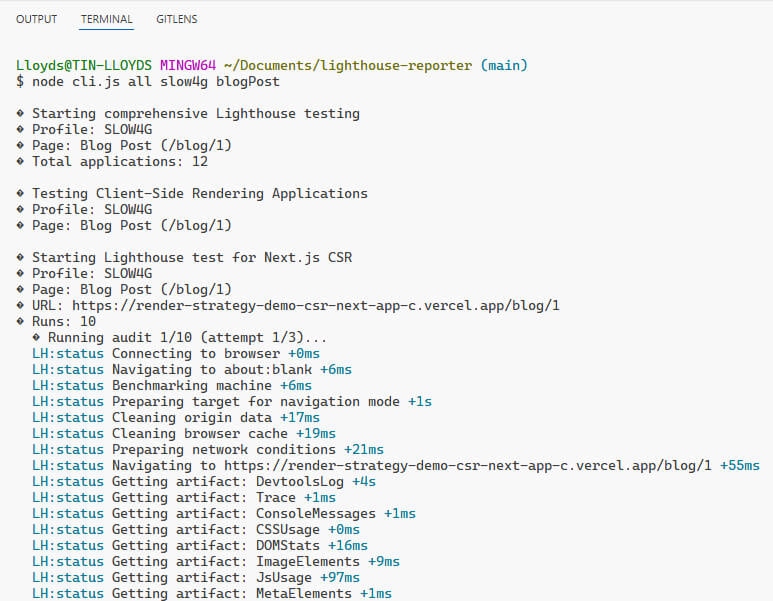
\includegraphics[width=\textwidth]{slike/metodologija/testiranje-aplikacije.jpg}
    \caption{Testiranje stranice pojedinog bloga kroz terminal}
    \label{fig:testiranje-aplikacije}
\end{figure}

\subsection{Struktura i prikaz podataka}

Prikupljeni podaci svake metrike dobivene CLI alatom Lighthouse pretvoreni su u mjerne jedinice prigodne za daljnju analizu i bolju interpretaciju rezultata. Npr. milisekunde su najprije pretvorene u sekunde, vrijednosti CLS (raspon od 0 do 1) su normalizirane i zaokružene na 3 decimale tako da se lakše uspoređuju između različitih testova. Uz izvorne vrijednosti u CSV datoteke s rezultatima pohranjene su i vrijednosti ocjene koju je tom rezultatu dodijelio Lighthouse.

\bigskip

Lighthouse svaki sirovi podatak pretvara u ocjenu od 0 do 100, gdje je 100 najbolja ocjena. Ovu ocjenu Lighthouse dodjeljuje na temelju krivulje distribucije izvedene iz stvarnih podataka o performansama web-stranica prikupljenih na HTTP Archiveu \cite
{chrome2025lighthouse}.

\bigskip

Budući da se prikaz rezulatata oslanja na ovu ocjenu Googleovog alata koja se prigodno izražava kao postotak, na većini grafova u ovom radu prikazane su ocjene učinka i postignuti rezulatati u obliku postotka. Uz određene rezultate prikazana je i standardna devijacija.

\subsection{Testno okruženje}

Kako bi se osigurali konzistentni uvjeti testiranja koji odgovaraju stvarnom korisničkom iskustvu, te omogućila podrška za specifične strategije iscrtavanja (kao što je ISR), odabran je sljedeći pristup.

\bigskip

Sve aplikacije postavljene su na platformu Vercel koja u trenutku pisanja ovog rada jedina podržava sve odabrane strategije iscrtavanja za svaki od prethodno navedenih programskih okvira. Ovo osigurava maksimalnu kompatibilnost i integraciju bez kompliciranih konfiguracija \cite{vercelframeworks}.

\bigskip

Vercel platforma također omogućava globalnu distribuciju putem CDN-a, što znači da se sadržaji serviraju iz čvorova najbližih korisniku. Zbog ovoga i činjenice da su sve aplikacije i njihov izvorni kod javno dostupni na Internetu, moguće je provođenje dodatnih istraživanja i proširivanja ovog rada, te osiguravanje relevantnosti podataka, bez obzira na geografsku lokaciju računala na kojem bi se potencijalno radila nova testiranja.
Testiranja provedena u ovom radu izvršena su na slijedećoj računalnoj konfiguraciji:

\bigskip

\begin{itemize}
    \item Model: Lenovo IdeaPad Slim 5 16ABR8
    \item Procesor: AMD Ryzen 5 7530U sa Radeon grafikom - 2.00 GHz
    \item Radna memorija: 16.0 GB (13.9 GB iskoristivo)
    \item Tip sustava: 64-bitni operacijski sustav, procesor baziran na arhitekturi x64
    \item Verzija operacijskog sustava: Windows 11 Home (24H2)
    \item Instalirana Node.js verzija: v22.14.0
\end{itemize}

Prije izvođenja testiranja zabilježeni su slijedeći mrežni uvjeti korištenjem Speedtest web alata:

\begin{itemize}
    \item Server: Tehnoline Telekom 45.142.9.180
    \item Ping: 15ms
    \item Jitter: 2ms
    \item Download: 291.6 Mbps
    \item Upload: 102.0 Mbps
\end{itemize}
